The first paper proposed the method LT-FH++, which is an extension of the previously proposed LT-FH method by Hujoel et al\cite{hujoel2020liability}. The notable difference between LT-FH and LT-FH++ is the ability to account for age of onset for cases or age for controls, sex, birth year, as well as the same information in the included family members. The LT-FH method considers parents in the same way and also does not distinguish between the index person and siblings, regardless of age differences or sex. Another difference is the ability to account for siblings individually rather than considering the number of siblings and an "\textit{at least one affected sibling}" indicator. This way of coding siblings in LT-FH is likely due to the way sibling information is coded in the UKBB. Considerable changes have also been made to the sampling strategy to allow for the increased flexibility in the family and their thresholds. The sampling strategy used for LT-FH would not work for LT-FH++, since LT-FH only needed to estimate a liability for each of the unique configurations. The changes LT-FH++ increased the number of unique configurations considerably, as each individual now has a unique set of family members and thresholds. 

\subsection{Simulation results}
We performed simulations to assess the power of LT-FH++ against LT-FH and a case control status to detect causal SNPs in a linear regression GWAS. The simulations are based on simulated genotypes, where we simulated a pair of parents and one offspring, meaning no siblings. The choice of parameters was heavily inspired by the ones used in the LT-FH paper to ensure compatibility between findings. The simulated genotypes had a heritability on the liability scale of $ h^2 = 0.5 $, a population prevalence of $ 5\% $, with a higher prevalence in one of the simulated sexes. The case ratio was $ 1:4 $ between sexes, and it was also present in the parents. We also considered a population prevalence of $ 10\% $, but they are not shown here. The genotypes consisted of $ 100,000 $ individuals, each with $ 100,000 $ independent SNPs where $ 1000 $ SNPs were causal, meaning an effect size different from $ 0 $. The simulations shown in \cref{fig:LTFHppSimulationResults} are based on $ 10 $ replications of the genotypes. Case ascertainment is common in biobanks, meaning a higher or lower prevalence of a phenotype of interest compared to the rest of the population. We emulated case ascertainment in the simulations by downsampling the entire population until it had a subpopulation with $ 10,000 $ individuals with a ratio of cases and control of $ 1:1 $.
\begin{figure}[h]
	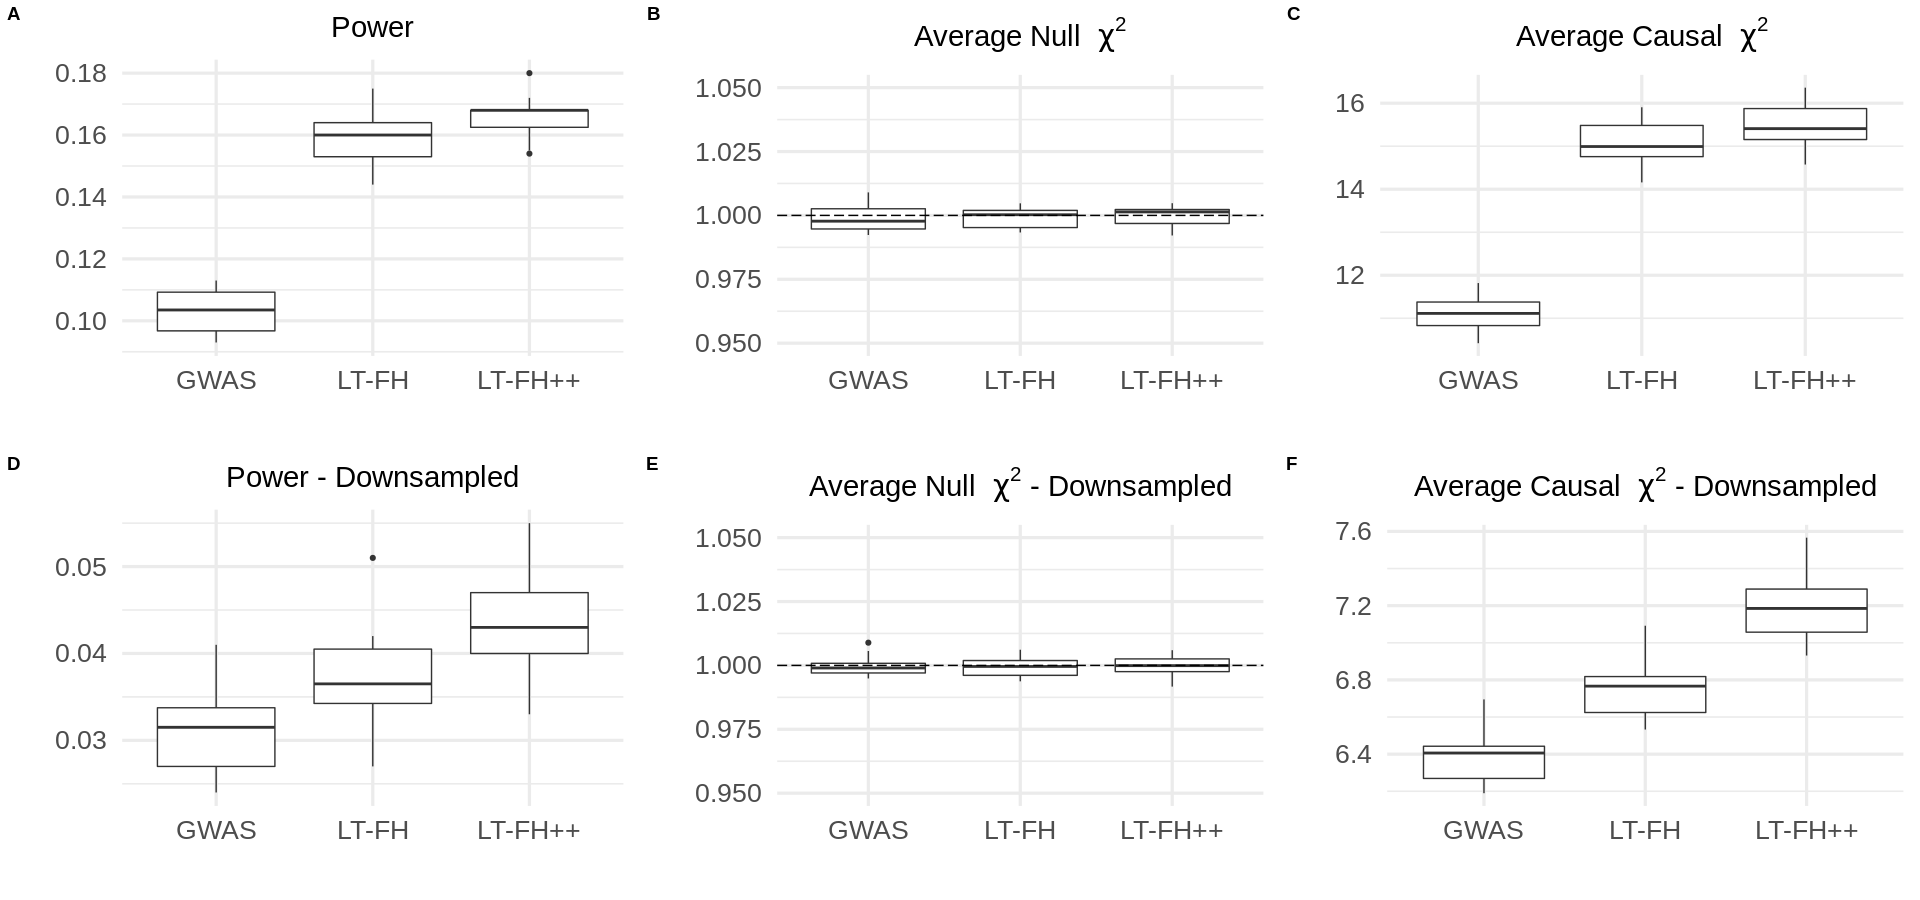
\includegraphics[width=\textwidth]{results/boxplot_05prev_both.pdf}
	\caption[Simulation results for a $ 5\% $ prevalence, with and without downsampling of controls]{Linear regression was used to perform the GWAS for LT-FH and LT-FH++, while a 1-df chi-squared test was used for case-control status. We assessed the power of each method by considering the fraction of causal SNPs with a p value below $ 5 \times 10^{-8} $. Here, GWAS refers to case-control status and LT-FH and LT-FH++ are both without siblings. Downsampling refers to downsampling the controls such that we have equal proportions of cases and controls, i.e., we have $ 10,000 $ individuals total for a $ 5\% $ prevalence and $ 20,000 $ individuals for a $ 10\% $ prevalence.}
	\label{fig:LTFHppSimulationResults}
\end{figure}

The simulations show a modest increase in favour of LT-FH++ over LT-FH in the full sample, with an average power increase across the $ 10 $ simulations of $ 4\% $. Both LT-FH and LT-FH++ has an average power increase of more than $ 50\% $ compared to the case-control status used in \texttt{GWAS}, making either method vastly better. However, case ascertainment has a significant impact on the power ratio between LT-FH and LT-FH++. When case ascertainment is present, the average power increase of LT-FH++ over LT-FH was $ 18\% $.

\newpage

\subsection{Real-world analysis}
\begin{wrapfigure}{O}{10cm}
	%	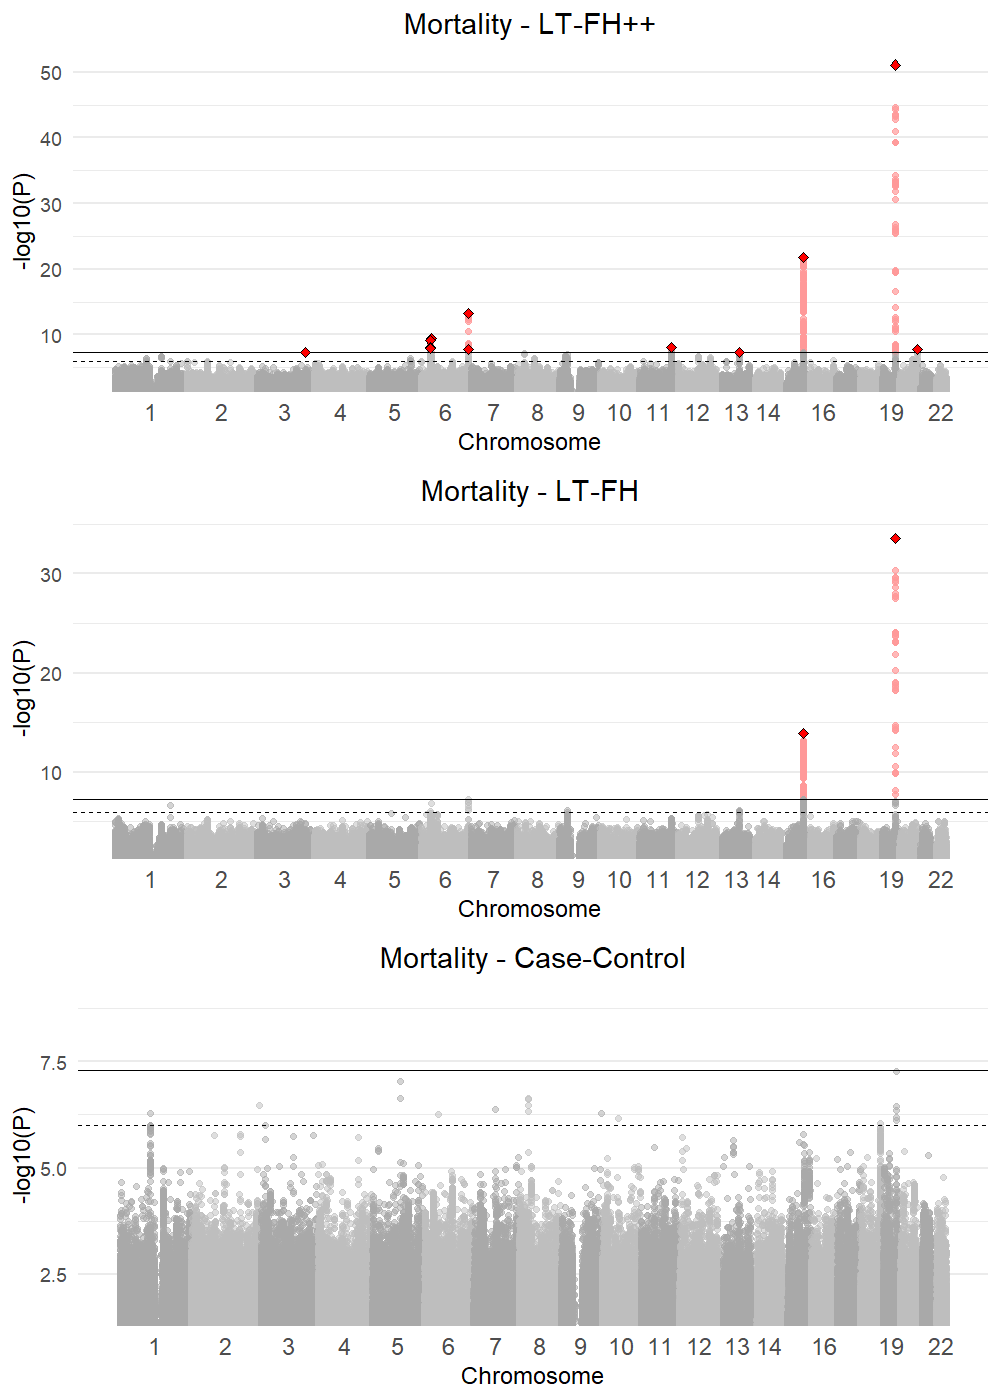
\includegraphics[width=0.7\textwidth]{results/manhattanPlot_mortality.pdf} % adds a lot of loading 
	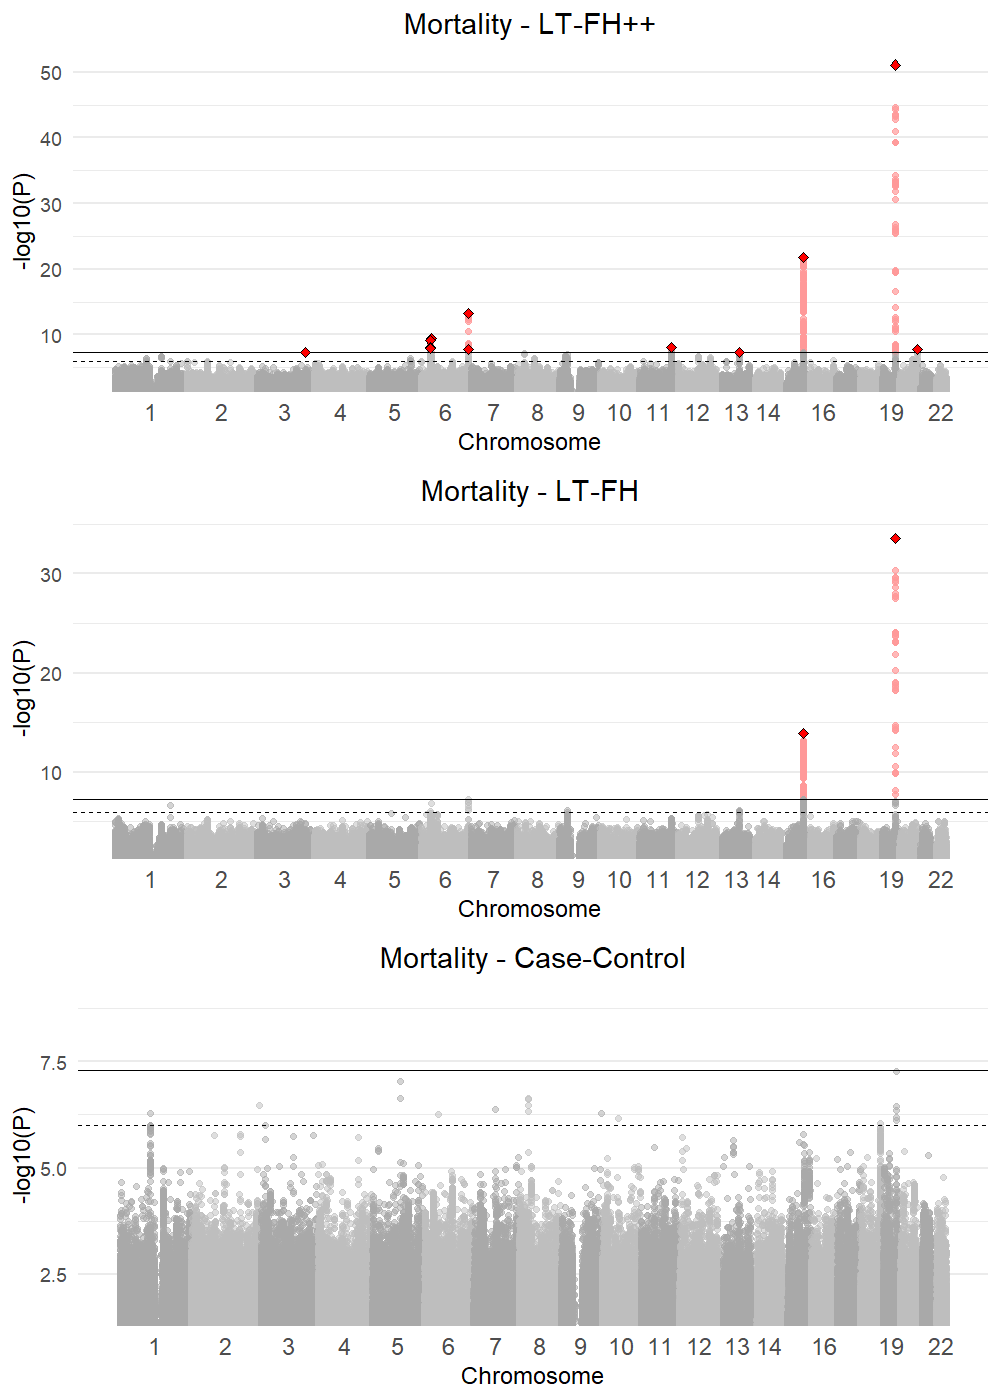
\includegraphics[width=10cm]{results/manhattanPlot_mortality.png}
	\caption[Manhattan plots for LT-FH++, LT-FH, and case-control GWAS of mortality	in the UK Biobank]{The Manhattan plots display a Bonferroni corrected significance level of $ 5\times 10^{-8} $ and a suggestive threshold of $ 5\times 10^{-6} $. The genome-wide significant SNPs are coloured in red. The diamonds correspond to top	SNPs in a window of size $ 300,000 $ base pairs.}
	\label{fig:LTFH++_manhattanMortality}
\end{wrapfigure}
LT-FH++ was also applied to four of the focus disorders of iPSYCH and mortality in UKBB. The mortality GWAS in UKBB resulted in $ 0 $ genome-wide significant SNP for simple linear regression, $ 2 $ for LT-FH, and $ 10 $ for LT-FH++. The Manhattan plot for mortality can be found in \cref{fig:LTFH++_manhattanMortality}.

The GWAS in iPSYCH did not provide nearly as large of an increase in power for LT-FH++ or LT-FH over simple linear regression. In fact, we did not see any notable improvement over simple linear regression of the case-control status. The Manhattan plot for ADHD in iPSYCH can be found in \cref{fig:LTFH++_manhattanADHD}. We did find $ 7 $ genome-wide significant SNPs for ADHD using LT-FH++ and $ 5 $ for LT-FH and case-control status, but the two additional associations for LT-FH++ were very close to genome-wide significance for the other two outcomes as well.
\begin{wrapfigure}{R}{10cm}
	%	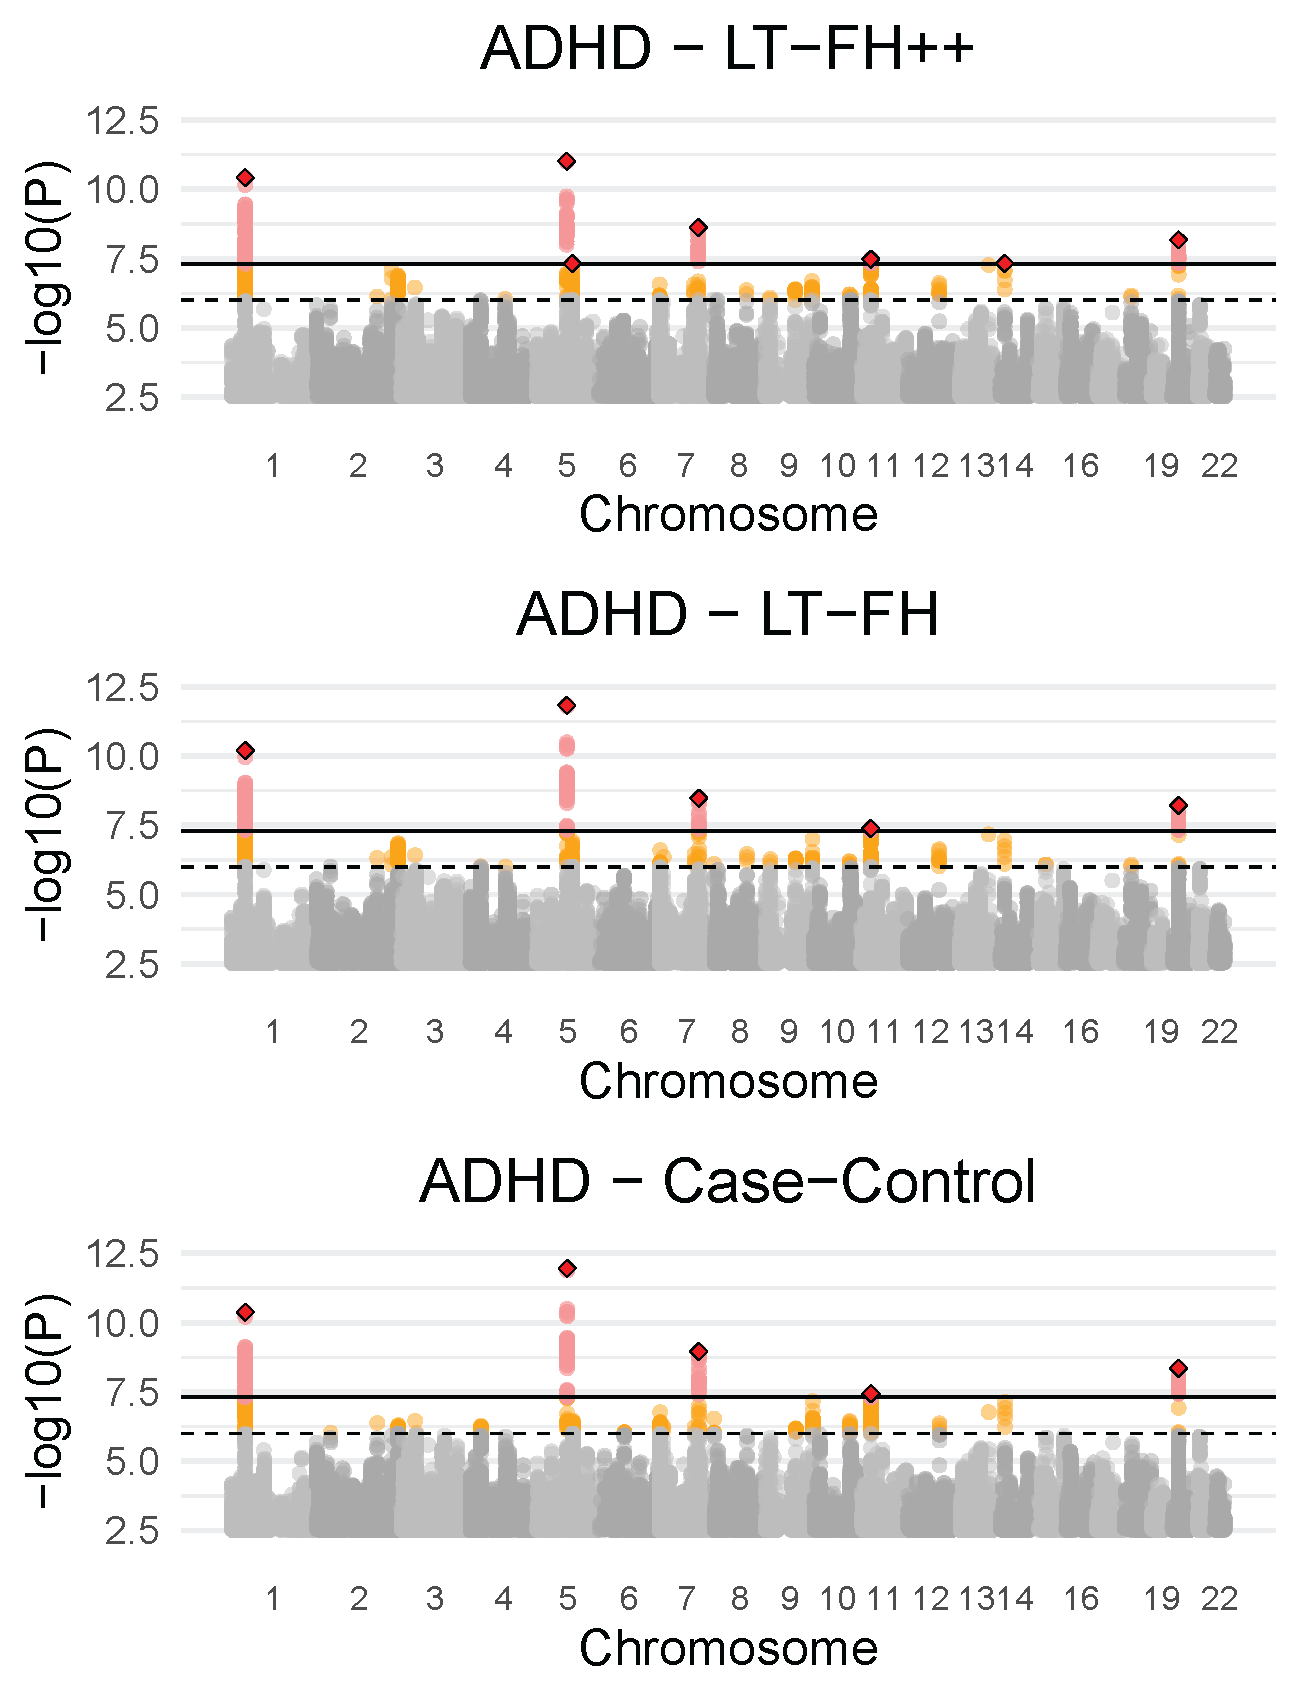
\includegraphics[width=0.7\textwidth]{results/manhattanPlot_ADHD.pdf} % adds a lot of loading 
	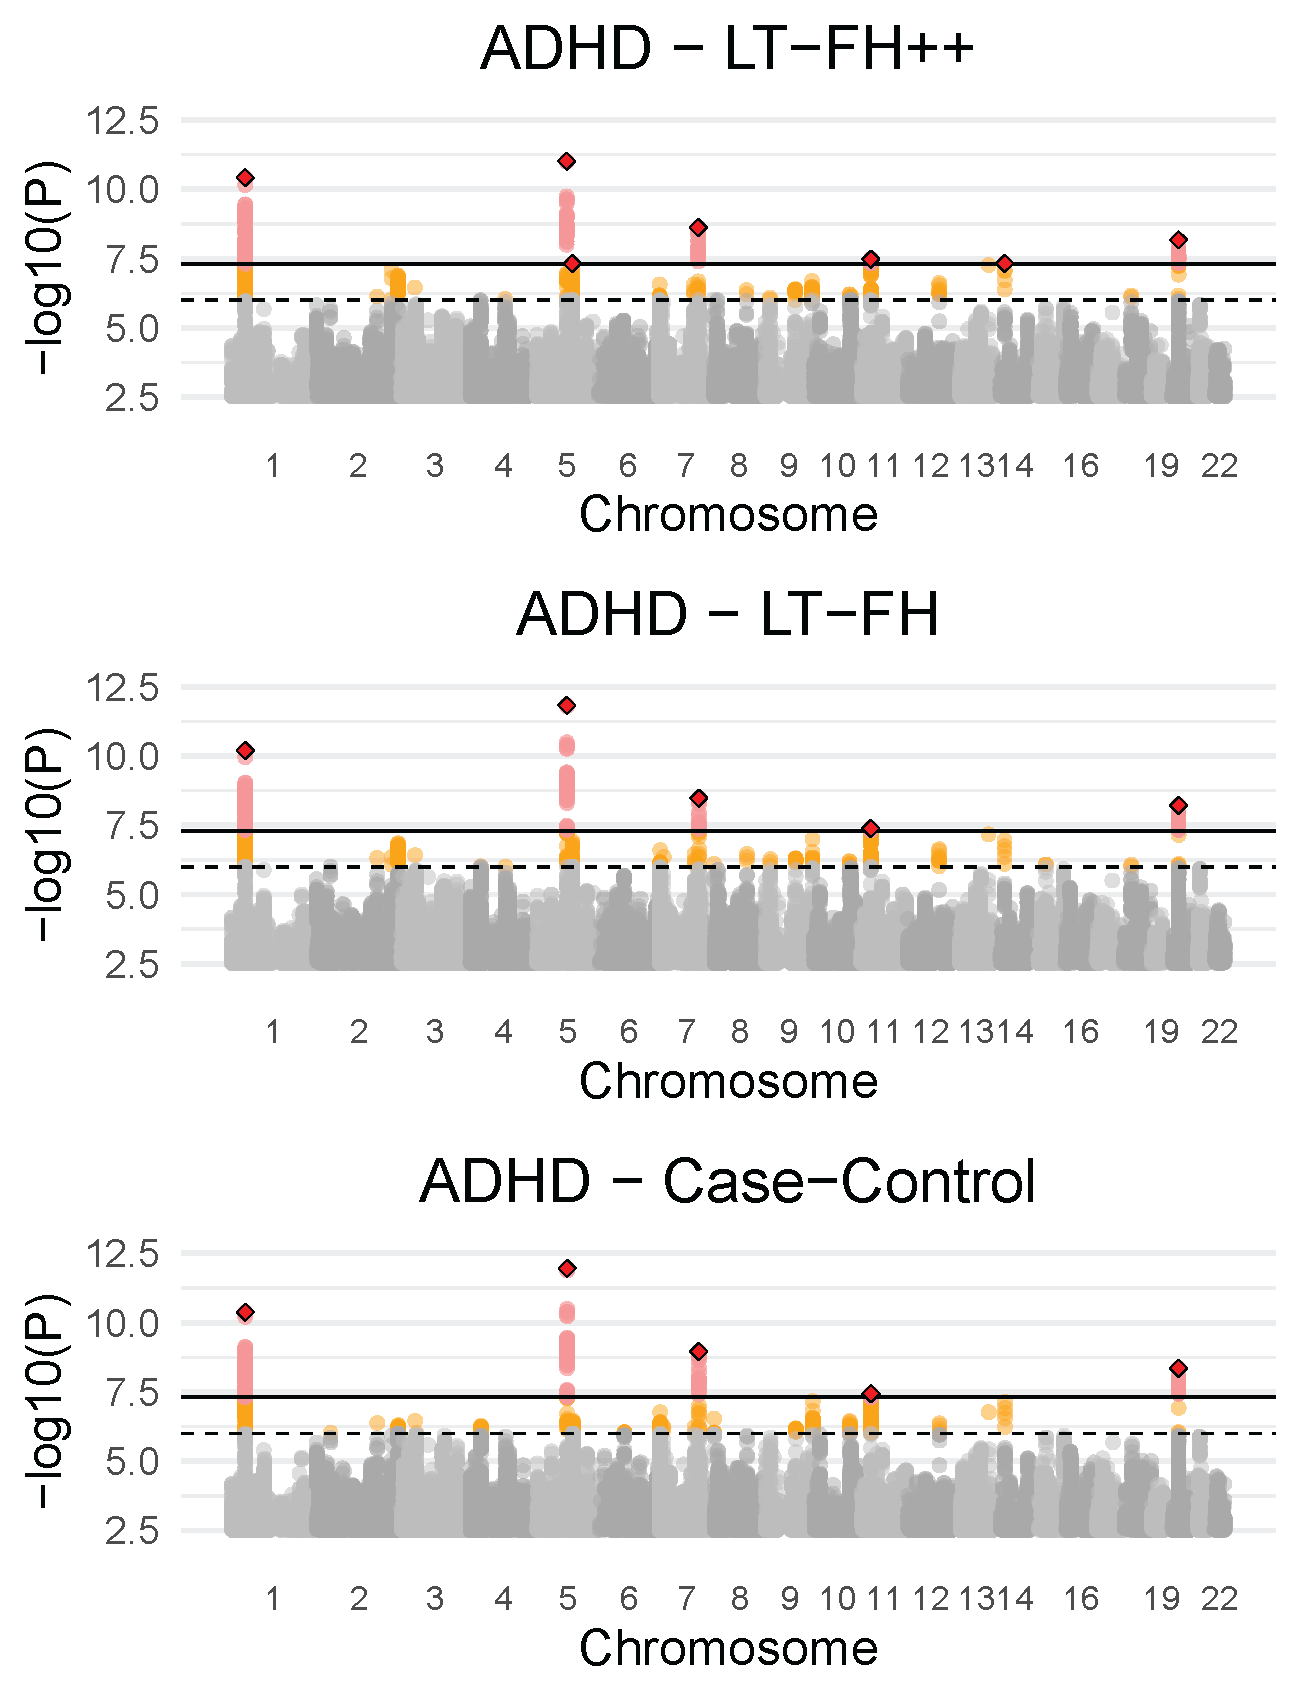
\includegraphics[width=10cm]{results/manhattanPlot_ADHD.png}
	\caption[Manhattan plots for LT-FH++, LT-FH, and case-control GWAS of ADHD in the iPSYCH data]{The dashed line indicates a suggestive p value of $ 5\times 10^{-6} $ and the fully drawn line at $ 5\times 10^{-8} $ indicates genome-wide significance threshold. The genome-wide significant SNPs are coloured in red. The diamonds correspond to top SNPs in a window of size $ 300,000 $ base pairs.}	
	\label{fig:LTFH++_manhattanADHD}
\end{wrapfigure}
Through additional simulations we found that one can expect the most \textit{relative} power gain with LT-FH++ over LT-FH if the in-sample prevalence is high in either family members or the index persons. This is due to the fact that LT-FH++ is best able to utilise information for cases, since the CIPs provide a very accurate estimate for the full liability of an individual.